\documentclass[mathserif,11pt]{beamer}


\setbeamercolor{block title}{bg=red!30,fg=black}

\mode<presentation>
{
\usetheme{default}
}


\title[] % (optional, use only with long paper titles)
{Automating Security Testing}
% \subtitle
% {Include Only If Paper Has a Subtitle}

\author[Therond, Therond]
{
  Eric~Therond
}

% Includes for frame package
\usepackage{framed,color}
\definecolor{shadecolor}{rgb}{0.5,0.5,0.5}

% Make a custom block
\newenvironment<>{customBlock}[1]{%
  \begin{actionenv}#2%
      \def\insertblocktitle{#1}%
      \par%
      \mode<presentation>{%
        \setbeamercolor{block title}{fg=white,bg=orange!20!black}
       \setbeamercolor{block body}{fg=black,bg=olive!50}
       \setbeamercolor{itemize item}{fg=orange!20!black}
       \setbeamertemplate{itemize item}[triangle]
     }%
      \usebeamertemplate{block begin}}
    {\par\usebeamertemplate{block end}\end{actionenv}}


% Define new environments for mdframed package
\usepackage{tikz}
\usepackage[framemethod=tikz]{mdframed}


\newmdenv[tikzsetting={draw=black,fill=white,fill opacity=0.7, line width=4pt},backgroundcolor=none,leftmargin=0,rightmargin=0,innertopmargin=4pt,skipbelow=\baselineskip,%
skipabove=\baselineskip]{TitleBox}
%http://tex.stackexchange.com/questions/38281/transparent-background-for-mdframed-environment

\usepackage{fontawesome} 

%----------------------------------------------------------------------------------------
\begin{document}

% My fancy title page, using transparent text box from mdframe, and icons from fontawesome
{  \usebackgroundtemplate{
\includegraphics[width=1.0\paperwidth]{background.jpg}}
  \begin{frame}[plain] 

  \vspace{15em}

  \begin{TitleBox}
    {\huge \inserttitle} 
    
    Eric Therond \href{mailto: contact@designsecurity.org}{{\FA \faEnvelope}  contact@designsecurity.org}\\
    {\footnotesize \href{https://fr.linkedin.com/in/eric-therond-2b320ba1}{{\FA \faLinkedinSign} Eric Therond}
    \href{http://www.designsecurity.org}{{\FA} http://www.designsecurity.org}
    }
   \end{TitleBox}

  \end{frame}
}

%Framed text examples
{
  \usebackgroundtemplate{
\includegraphics[width=2.0\paperwidth]{bg.jpg}}
  \begin{frame}[plain] 

\setbeamercolor{block title}{use=structure,fg=white,bg=black!60}
\setbeamercolor{block body}{use=structure,fg=black,bg=white!60!white}

\begin{block}{What kinds of security tests can be automated ?}
\begin{itemize}
\item Part of security tests is subjective
  \begin{itemize}
  \item Acquire confidence about a service
  \item Measure robustness of a service against experimented hackers
  \end{itemize}
\end{itemize}

\begin{itemize}
\item Security tests coverage should include measure of
  \begin{itemize}
  \item The legitimacy to collect and process personal data
  \item The eligibility for access to classified information
  \end{itemize}
\end{itemize}

\begin{itemize}
\item It's difficult to test stakeholders expectatives.
\item So detection of known vulnerabilities is our first goal.
\end{itemize}
\end{block}

  \end{frame}
}

{
  \usebackgroundtemplate{
\includegraphics[width=2.0\paperwidth]{bg.jpg}}
  \begin{frame}[plain] 

\setbeamercolor{block title}{use=structure,fg=white,bg=black!60}
\setbeamercolor{block body}{use=structure,fg=black,bg=white!60!white}

\begin{block}{How security tests can be automated ?}
\begin{itemize}
\item Automating security testing is a \textbf{cost project} : you need skilled and experimented QA for developping process, tools and documentation.
\item An exploit which could be used to test the presence of heartbleed openssl vulnerability is about 700 lines of low level code : https://www.exploit-db.com/exploits/32791/
\item More than 5000 new vulnerabilities are referenced each year : http://www.cvedetails.com/browse-by-date.php
\item We are going to use open-source tools to test the exposure of organizations against those common vulnerabilities.
\item It's a necessary step but for reasons invoked earlier it's not sufficient : 
\begin{itemize}
\item Each organization has his own known, specifics and legacies vulnerabilities which must be tested regularly.
\item Deeper analysis like intensives codes reviews and penetrations tests are the basics for criticals systems.
\end{itemize}
\end{itemize}
\end{block}

  \end{frame}
}

{
  \usebackgroundtemplate{
\includegraphics[width=2.0\paperwidth]{bg.jpg}}
  \begin{frame}[plain] 

\setbeamercolor{block title}{use=structure,fg=white,bg=black!60}
\setbeamercolor{block body}{use=structure,fg=black,bg=white!60!white}

\begin{block}{What are the benefits of automated security tests ?}
\begin{itemize}
\item Improve the coverage of systems under testing.
\item Security experts are forsaken of manuals and repetitives tasks.
\item You need a process for automating tests (developers and administrators are directly impliqued in the running of tests and remediations of detected defaults, SOC are correlated with security testing) and so the maturity of organizations increases quickly.
\item Automated security tests are the first attacks that a hacker will doing against your organization, your knowledge of these techniques will help you to identify and block your attackers.
\end{itemize}
\end{block}

  \end{frame}
}

{
  \usebackgroundtemplate{
\includegraphics[width=2.0\paperwidth]{bg.jpg}}
  \begin{frame}[plain] 

\setbeamercolor{block title}{use=structure,fg=white,bg=black!60}
\setbeamercolor{block body}{use=structure,fg=black,bg=white!60!white}


\begin{block}{Illustrated Solution}
\begin{center}
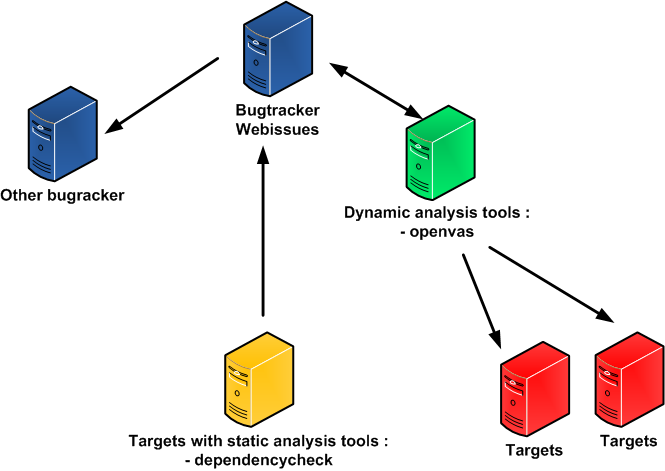
\includegraphics[scale=0.45]{prezsec1.png}
\end{center}
\end{block}
    
  \end{frame}
}


{
  \usebackgroundtemplate{
\includegraphics[width=2.0\paperwidth]{bg.jpg}}
  \begin{frame}[plain] 

\setbeamercolor{block title}{use=structure,fg=white,bg=black!60}
\setbeamercolor{block body}{use=structure,fg=black,bg=white!60!white}

\begin{block}{Add servers}
\begin{center}
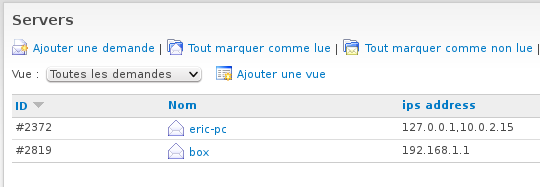
\includegraphics[scale=0.7]{prezsec2.png}
\end{center}
\end{block}

\begin{block}{Detailed Solution}
\begin{itemize}
\item Project servers are added with the HIM or WebService.
\item Each server can have multiple ips.
\item These servers will be scan by dynamic analysis tools.
\item By default the tool is OpenVas.
\end{itemize}
\end{block}

  \end{frame}
}

{
  \usebackgroundtemplate{
\includegraphics[width=2.0\paperwidth]{bg.jpg}}
  \begin{frame}[plain] 

\setbeamercolor{block title}{use=structure,fg=white,bg=black!60}
\setbeamercolor{block body}{use=structure,fg=black,bg=white!60!white}

\begin{block}{Add codes}
\begin{center}
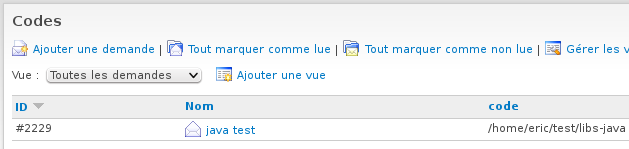
\includegraphics[scale=0.55]{prezsec3.png}
\end{center}
\end{block}

\begin{block}{Detailed Solution}
\begin{itemize}
\item Project codes are added with the HIM or WebService.
\item Each code has a path.
\item These paths will be scan by static analysis tools.
\item By default the tool is DependencyCheck.
\end{itemize}
\end{block}

  \end{frame}
}


{
  \usebackgroundtemplate{
\includegraphics[width=2.0\paperwidth]{bg.jpg}}
  \begin{frame}[plain] 

\setbeamercolor{block title}{use=structure,fg=white,bg=black!60}
\setbeamercolor{block body}{use=structure,fg=black,bg=white!60!white}

\begin{block}{Run a scan}
\begin{center}
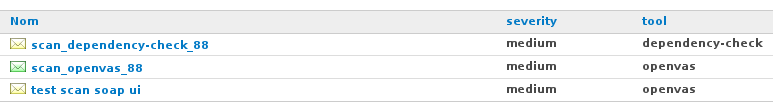
\includegraphics[scale=0.5]{prezsec4.png}
\end{center}
\end{block}

\begin{block}{Detailed Solution}
\begin{itemize}
\item Run scan with the HIM or WebService.
\item All ips address in the folder servers will be scan.
\item All paths codes in the folder codes will be scan.
\item Filter as severity of bugs can be specified.
\item When OpenVas finish a scan an alert is sent to the bugtracker and detected bugs are recorded in the associated folder.
\end{itemize}
\end{block}

  \end{frame}
}


{
  \usebackgroundtemplate{
\includegraphics[width=2.0\paperwidth]{bg.jpg}}
  \begin{frame}[plain] 

\setbeamercolor{block title}{use=structure,fg=white,bg=black!60}
\setbeamercolor{block body}{use=structure,fg=black,bg=white!60!white}

\begin{block}{View bugs}
\begin{center}
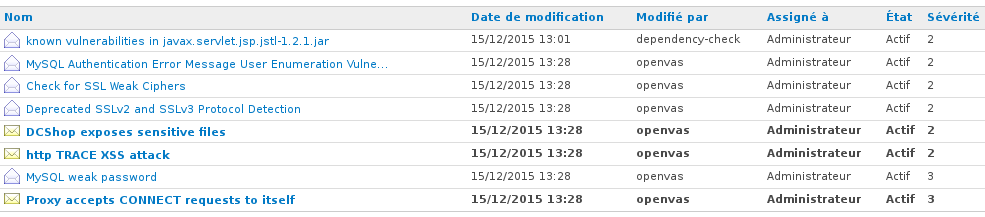
\includegraphics[scale=0.4]{prezsec5.png}
\end{center}
\end{block}

\begin{block}{Detailed Solution}
\begin{itemize}
\item View bugs with the HIM or WebService.
\item The creator of the bug is the analysis tool.
\item By default the bug is assigned to an administor of the project.
\end{itemize}
\end{block}

  \end{frame}
}

{
  \usebackgroundtemplate{
\includegraphics[width=2.0\paperwidth]{bg.jpg}}
  \begin{frame}[plain] 

\setbeamercolor{block title}{use=structure,fg=white,bg=black!60}
\setbeamercolor{block body}{use=structure,fg=black,bg=white!60!white}


\begin{block}{Continuous Integration}
\begin{itemize}
\item Other analysis tools can be used.
\item All the methods can be used via Web Service.
\item Duplicated bugs are handled.
\item Bugs can be move to another bugtracker.
\item Jobs in link with configuration management can be used :
\item With Jenkins FSTrigger plugin you can Monitor file system when a server is added for example and run dynamic analysis scan (jobs/run\_openvas.php).
\end{itemize}
\end{block}

  \end{frame}
}
% Example using built-in title functions
{
 \usebackgroundtemplate{
\includegraphics[width=2.0\paperwidth]{bg.jpg}}
  \begin{frame}[plain] 

  \begin{TitleBox} {
    \begin{center}
      \huge \inserttitle \\
      \small{
      26/02/2016\\
      Webinar build security - DesignSecurity\\
      https://github.com/eric-therond/security-bugtracker}
      \end{center}
      } 
  \end{TitleBox}

  \end{frame}
}


%-----------------------------------
\end{document} 
